\documentclass[12pt]{article}
\usepackage[english]{babel}
\usepackage{float}
\usepackage[margin=1in]{geometry}
\usepackage{graphicx}
%\usepackage[toc,page]{appendix}
\graphicspath{ {./doc/img/} }
\newcommand{\rpm}{\raisebox{.2ex}{$\scriptstyle\pm$}} 
\usepackage{listings}
\usepackage{xcolor}
\usepackage{indentfirst}
\usepackage[final]{pdfpages}


\begin{document}

\title{Joe Phaneuf \\ Computer Vision 16-720 Spring 2018 \\ Feb. 03, 2018 }
\date{}
\author{}
\maketitle

\newpage


\stepcounter{section}
\section{Theory Questions}

\subsection{}
Mapping a point in image space $(x,y)$ to Hough space, $x$ and $y$ become constants.  
$\rho(\theta) = x cos \theta + y sin \theta$  
Being a linear combination of same-period sinusoids, $\rho(\theta)$ is guaranteed to be a sinusoid.  

\newpage
\subsection{}
Hough space can be parameterized in slope-intercept form.  
Doing so creates two major problems:  

\begin{itemize}
\item The slope and intercept parameters are unbounded, making implementation impractical
\item Vertical lines (infinite slope) cannot be represented 
\end{itemize}


When parameterizing in normal form, the magnitude and angle are bounded (magnitude bound is a function of image size).

$\rho = x cos \theta + y sin \theta$  
$y sin \theta = \rho - x cos \theta$  
$y = - \frac{1}{tan \theta} x + \frac{\rho}{sin \theta}$  
$m =- \frac{1}{tan \theta}$ , $c = \frac{\rho}{sin \theta}$  

\newpage
\subsection{}
The range of $\theta$ is independent on image size: $- \frac{\pi}{2} \leq \theta \leq \frac{\pi}{2}$  
The largest $\rho$ will be a diagonal across the image space: $0 \leq abs(\rho) \leq \sqrt{W^{2} + H^{2}}$

\newpage
\subsection{}
\textbf{Matlab script for plot generation in matlab: q2.4.m}

Image space points (10, 10), (15, 15) and (30, 30) were represented in Hough space, resulting in sinusoids as discussed above. The sinusoids in Hough space intersect at one point. That point describes a line in image space that passes through the points (10, 10), (15, 15) and (30, 30). The sinusoids intersect at $\theta = - \frac{pi}{4}$ , $\rho = 0$, which describes a 45 degree line passing through origin in image space, i.e. $m=1$, $c=0$.



\begin{figure}[H]
\centering
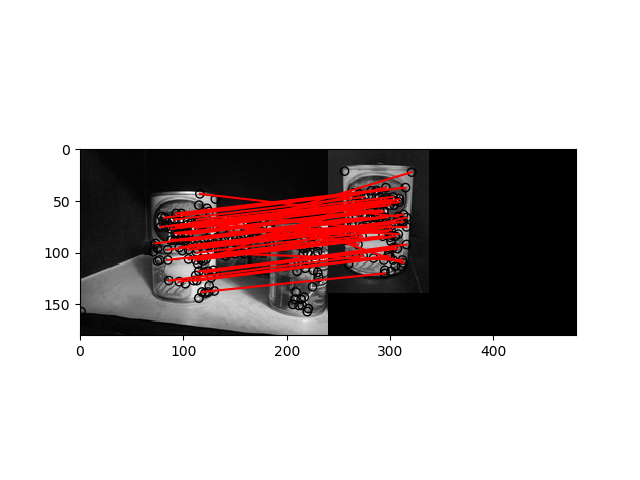
\includegraphics[page=1,width=0.75\textwidth]{q2_4}
\caption{Intersecting lines in Hough space}    
\label{fig:intersect_hough}
\end{figure}   

\newpage
\section{Implementation}
\begin{figure}[H]
\centering
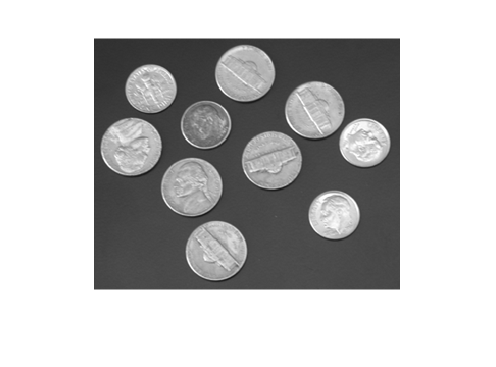
\includegraphics[page=1,width=0.75\textwidth]{coins}
\caption{Original image for implementation test}    
\label{fig:intersect_hough}
\end{figure}   

\subsection{}
\begin{figure}[H] \centering 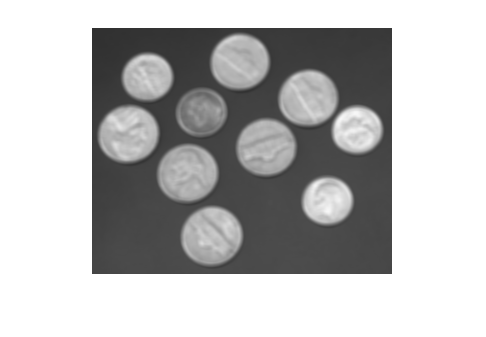
\includegraphics[page=1,width=0.75\textwidth]{imagefilter_blur}
\caption{Blurred image using myImageFilter}    \end{figure}   


\newpage
\subsection{}
I chose to implement the image filter with a single for loop. In essence, the for loop loops through each pixel (nrows*ncols), and for each pixel uses divides/modulos to determine neighboring pixels.

\newpage
\subsection{}
\begin{figure}[H] \centering 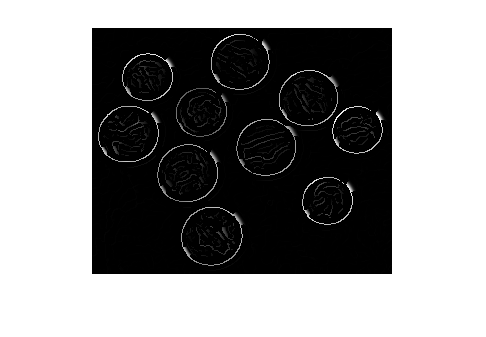
\includegraphics[page=1,width=0.75\textwidth]{edgefilter_im}
\caption{Edge filter magnitude}    \end{figure}   
\begin{figure}[H] \centering 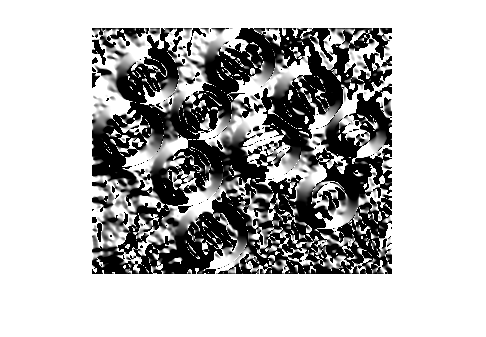
\includegraphics[page=1,width=0.75\textwidth]{edgefilter_io}
\caption{Edge filter orientation}    \end{figure}   
\begin{figure}[H] \centering 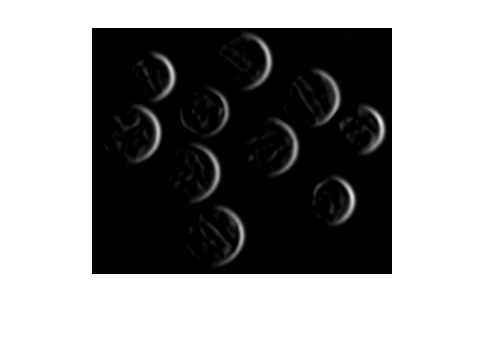
\includegraphics[page=1,width=0.75\textwidth]{edgefilter_ix}
\caption{Edge filter gradient x}    \end{figure}   
\begin{figure}[H] \centering 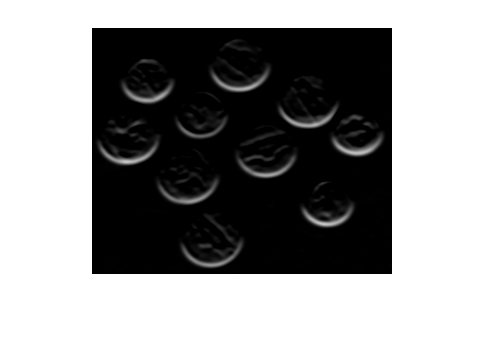
\includegraphics[page=1,width=0.75\textwidth]{edgefilter_iy}
\caption{Edge filter gradient y}    \end{figure}   


\newpage
\subsection{}
\begin{figure}[H] \centering 
\includegraphics[page=1,width=0.75\textwidth]{hough}
\caption{Hough transform}    \end{figure}   


\newpage
\subsection{}
\begin{figure}[H] \centering 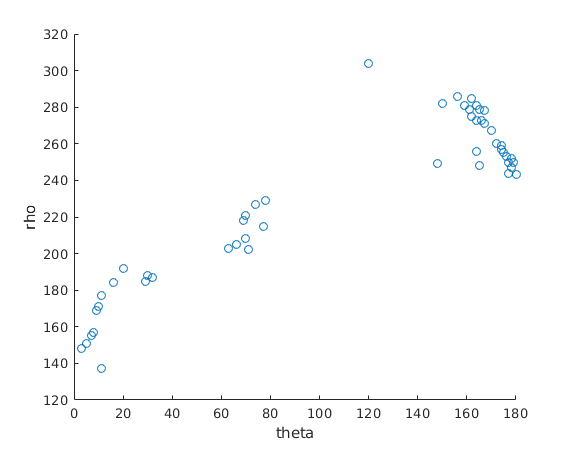
\includegraphics[page=1,width=0.75\textwidth]{thetas_rhos}
\caption{Hough line parameters}    \end{figure}   


\newpage
\subsection{}
\begin{figure}[H] \centering 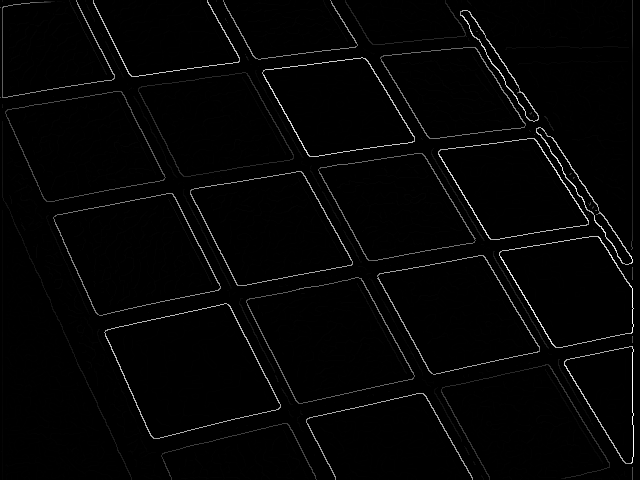
\includegraphics[page=1,width=0.75\textwidth]{img01_01edge}
\caption{Image 1 edges}    \end{figure}   
\begin{figure}[H] \centering 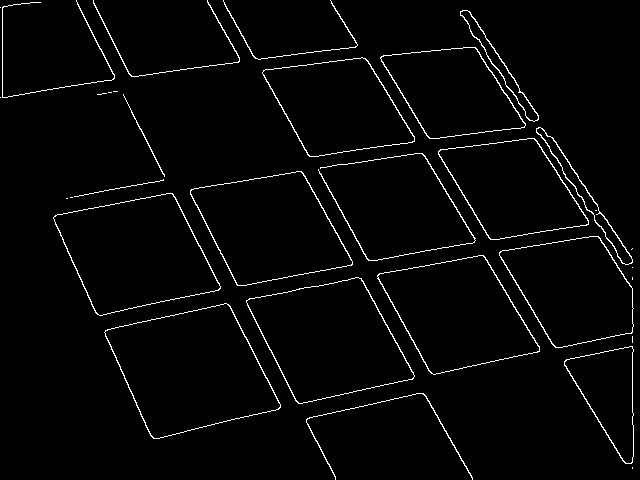
\includegraphics[page=1,width=0.75\textwidth]{img01_02threshold}
\caption{Image 1 thresholded}    \end{figure}   
\begin{figure}[H] \centering 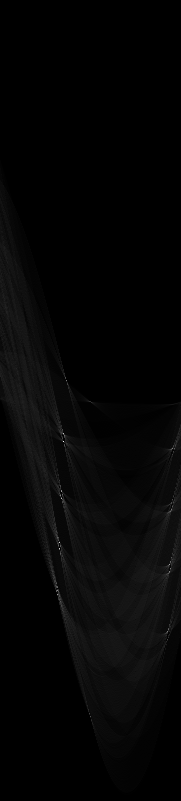
\includegraphics[page=1,width=0.75\textwidth]{img01_03hough}
\caption{Image 1 Hough transform}    \end{figure}   
\begin{figure}[H] \centering 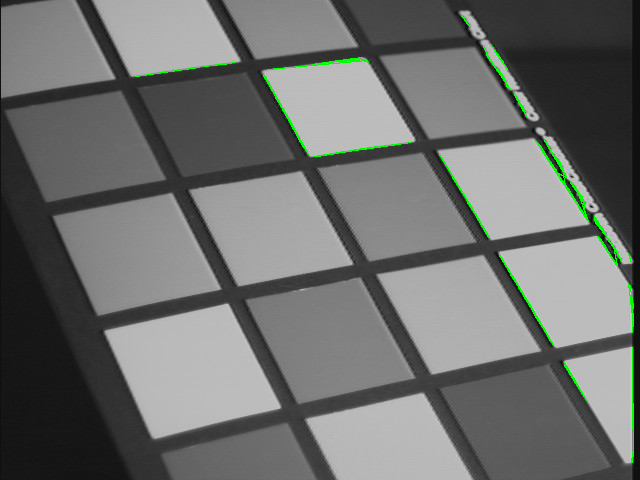
\includegraphics[page=1,width=0.75\textwidth]{img01_04lines}
\caption{Image 1 lines fitted}    \end{figure}   


\newpage
\section{Experiments}
\subsection{Cross image performance}
I was unable to find a single set of parameters that performered equally well across all images.

\newpage
\subsection{Optimal parameters}
After experimenting on 10 parameter sets, the gaussian filter standard deviation parameter appears to have the most impact on image to image variation. Experiments with lower standard deviation showed better results for images with clearly defined lines and little noise (such as image 1), however noisier images (such as image 6 and image 9) had noisy responses.
Increasing the standard deviation of the gaussian filter results in cleaner lines on noisy images, but resulted in fewer detected lines on less noisy images.

\newpage
\subsection{Problematic steps}
From these results I would argue the the edge filter is the most problematic piece of this process, as a fixed blur causes inconsistent results across images with wildly different frequency content.

\newpage
\subsection{Performance increases}
I found maintaining single for loops / vectorization to provide faster performance when batch processing images.

\newpage
\subsection{Tabulate experiments}

\subsubsection{}
\begin{tabular} { c c }
Name  &  31January2018:10:57:11 \\
sigma  &  2.000000 \\
threshold  &  0.030000 \\
rhoRes & 2.000000 \\
thetaRes & 0.034907 \\
nLines & 50.000000 
\end{tabular}
\\ \\
These parameters work poorly on all images.

\subsubsection{}
\begin{tabular} { c c }
Name & 31January2018:12:18:43\\
sigma & 2.000000\\
threshold & 0.030000\\
rhoRes & 2.000000\\
thetaRes & 1.000000\\
nLines & 50.000000
\end{tabular}
\\ \\
These parameters perform approximately as well as the initial parameters, however increasing angular step size reduces computation time dramatically.

\subsubsection{}
\begin{tabular} { c c }
Name & 31January2018:12:29:22\\
sigma & 2.000000\\
threshold & 0.500000\\
rhoRes & 2.000000\\
thetaRes & 1.000000\\
nLines & 50.000000
\end{tabular}
\\ \\
Increasing the threshold resulted in much more accurate lines on all images, however on most images the algorithm was unable to match up to nLines.

\subsubsection{}
\begin{tabular} { c c }
Name & 31January2018:12:40:05\\
sigma & 2.000000\\
threshold & 0.250000\\
rhoRes & 1.000000\\
thetaRes & 1.000000\\
nLines & 50.000000
\end{tabular}
\\ \\
Dropping the the threshold by half and using finer magnitude step size did not dramatically change results.

\subsubsection{}
\begin{tabular} { c c }
Name & 31January2018:12:49:09\\
sigma & 1.000000\\
threshold & 0.100000\\
rhoRes & 1.000000\\
thetaRes & 1.000000\\
nLines & 50.000000
\end{tabular}
\\ \\
Dropping threshold to 0.1 and reducing blur results in decreased accuracy on noisy and non-linear images.

\subsubsection{}
\begin{tabular} { c c }
Name & 31January2018:12:53:47\\
sigma & 1.000000\\
threshold & 0.250000\\
rhoRes & 1.000000\\
thetaRes & 1.000000\\
nLines & 50.000000
\end{tabular}
\\ \\
Increasing threshold back to 0.25 has little effect, noisy and non-linear images have poor results.

\subsubsection{}
\begin{tabular} { c c }
Name & 31January2018:13:16:10\\
sigma & 3.000000\\
threshold & 0.500000\\
rhoRes & 1.000000\\
thetaRes & 5.000000\\
nLines & 50.000000
\end{tabular}
\\ \\
Trying more blur and reducing angular resolution with a high threshold produces too few lines on all images, though the lines are accurate.

\subsubsection{}
\begin{tabular} { c c }
Name & 31January2018:13:17:32\\
sigma & 3.000000\\
threshold & 0.100000\\
rhoRes & 1.000000\\
thetaRes & 5.000000\\
nLines & 50.000000
\end{tabular}
\\ \\
Reducing threshold and maintaining high blur produces relatively consistent performance across the image set.

\subsubsection{}
\begin{tabular} { c c }
Name & 31January2018:15:12:35\\
sigma & 3.000000\\
threshold & 0.100000\\
rhoRes & 1.000000\\
thetaRes & 0.500000\\
nLines & 50.000000
\end{tabular}
\\ \\
Finer angular resolution has a small improvement on performance. This is the most consistently well performing parameter set I was able to produce.

\newpage
\subsection{Performance across images, effect of parameters}
Images with non-linear elements (such as image 2 with the vase and image 6 with the text on boxes) consistently resulted in inaccurate lines. Increasing the edge threshold resulted in fewer but more accurate lines on these images.

\end{document}



